\documentclass[a4paper,12pts]{article}
\usepackage[margin=.6in]{geometry}
\usepackage{amsmath,amssymb,amsfonts}
\usepackage{cancel}
\usepackage{graphicx}
\usepackage{float}
\title{\textbf{\Huge{Assignment 1}}}
\author{\Large{Name : Harshit Pant}\\\Large{Roll Number : CS21BTECH$11021$}}
\date{}
\begin{document}
\maketitle
\setlength{\parindent}{0cm}
\textbf{Q.6(c) [ICSE 2018] :}
Prove that $(1 +\cot\theta -\csc\theta)(1 + \tan\theta +\sec\theta)=2$\\

\textbf{Solution : }
\begin{align*}
(1+ \cot\theta -\csc\theta)(1+\tan\theta+\sec\theta)&=(1+\cot\theta-\csc\theta)+\tan\theta(1+\cot\theta-\csc\theta)+\sec\theta(1+\cot\theta-\csc\theta)\\[.1in]
\begin{split}
(1+ \cot\theta -\csc\theta)(1+\tan\theta+\sec\theta)&=1+\cot\theta-\csc\theta+\tan\theta+\tan\theta\times\cot\theta-\tan\theta\times\csc\theta+\sec\theta\\[.1in]
&\qquad
+\sec\theta\times\cot\theta-\sec\theta\times\csc\theta
\end{split}\\[.1in]
\begin{split}
(1+ \cot\theta -\csc\theta)(1+\tan\theta+\sec\theta)&=\displaystyle{1+\cot\theta-\csc\theta+\tan\theta+1-\frac{\cancel{\sin\theta}}{\cos\theta}\times\frac{1}{\cancel{\sin\theta}}+\sec\theta+\frac{1}{\cancel{\cos\theta}}\times\frac{\cancel{\cos\theta}}{\sin\theta}}\\[.1in]
&\qquad
-\sec\theta\times\csc\theta
\end{split}
\\[.1in]
(1+ \cot\theta -\csc\theta)(1+\tan\theta+\sec\theta)&=1+\cot\theta-\cancel{\csc\theta}+\tan\theta+1-\cancel{\sec\theta}+\cancel{\sec\theta}+\cancel{\csc\theta}-\sec\theta\times\csc\theta\\[.1in]
(1+ \cot\theta -\csc\theta)(1+\tan\theta+\sec\theta)&=2+\dfrac{\cos\theta}{\sin\theta}+\dfrac{\sin\theta}{\cos\theta}-\sec\theta\times\csc\theta\\[.1in]
(1+ \cot\theta -\csc\theta)(1+\tan\theta+\sec\theta)&=\displaystyle{2+\dfrac{{\cos}^2\theta+{\sin}^2\theta}{\sin\theta\times\cos\theta}-\sec\theta\times\csc\theta}\\[.1in]
(1+ \cot\theta -\csc\theta)(1+\tan\theta+\sec\theta)&=\displaystyle{2+\frac{1}{\sin\theta\times\cos\theta}-\sec\theta\times\csc\theta}\hspace{1in}
(\because{\cos}^2\theta+{\sin}^2\theta=1)\\[.1in]
(1+ \cot\theta -\csc\theta)(1+\tan\theta+\sec\theta)&=\displaystyle{2+\cancel{\csc\theta\times\sec\theta}-\cancel{\sec\theta\times\csc\theta}}\\[.1in]
(1+ \cot\theta -\csc\theta)(1+\tan\theta+\sec\theta)&=2\\
\text{L.H.S}&=\text{R.H.S}
\end{align*}
\\[.03in]
Hence proved.\\[.1in]
\textbf{\Large{Output}}
\begin{figure}[H]
\begin{center}
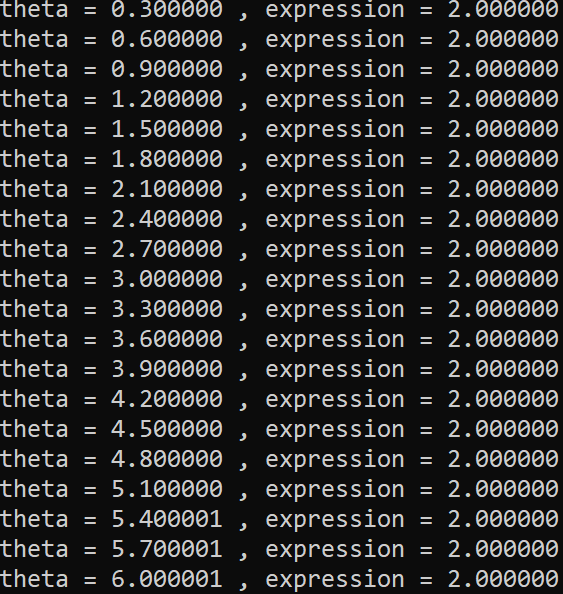
\includegraphics[width=2.5in]{fig.png}
\end{center}
\end{figure}

\end{document}
